%%%%%%%%%%%%%%%%%%%%%%%%%%%%%%%%%%%%%%%%%%%%%%%%%%%%%%%%%%%%%%%%%%%%%%%%%%%%%%%%
%2345678901234567890123456789012345678901234567890123456789012345678901234567890
%        1         2         3         4         5         6         7         8

\documentclass[letterpaper, 10 pt, conference]{ieeeconf}  % Comment this line out if you need a4paper

%\documentclass[a4paper, 10pt, conference]{ieeeconf}      % Use this line for a4 paper

\IEEEoverridecommandlockouts                              % This command is only needed if 
                                                          % you want to use the \thanks command

\overrideIEEEmargins                                      % Needed to meet printer requirements.

% See the \addtolength command later in the file to balance the column lengths
% on the last page of the document

% The following packages can be found on http:\\www.ctan.org
%\usepackage{graphics} % for pdf, bitmapped graphics files
%\usepackage{epsfig} % for postscript graphics files
%\usepackage{mathptmx} % assumes new font selection scheme installed
%\usepackage{times} % assumes new font selection scheme installed
\usepackage{amsmath} % assumes amsmath package installed
%\usepackage{amssymb}  % assumes amsmath package installed
\usepackage{bm}  % assumes bm package installed
\usepackage{graphicx}
\usepackage[font=footnotesize]{subcaption}
%\usepackage{siunitx}
\usepackage{amssymb}
\usepackage{cuted}
\usepackage{xcolor}
%\usepackage{ngerman}
\usepackage[utf8]{inputenc}
%\usepackage{onimage}
\usepackage{algorithm2e}
\usepackage{overpic}
\captionsetup{font=footnotesize}
%\usepackage[draft]{changes}

% Leerräume stauchen
\renewcommand{\baselinestretch}{0.89}


% !TEX root = collhdl_ICRA_17.tex

\title{\LARGE \bf
Collision Detection, Isolation and Identification for Humanoids
}

\author{Jonathan Vorndamme, Moritz Schappler and Sami Haddadin$^{1}$
% <-this % stops a space
\thanks{$^{1}$The authors are members of the Institute of Automatic Control at Leibniz Universit\"at Hannover, {\tt\small lastname@irt.uni-hannover.de}.
\newline
This work has been partially funded by the
European Union’s Horizon 2020 research and innovation programme under grant agreement No 688857 (``SoftPro'') and by the Alfried-Krupp Award for young professors.}
}

\begin{document}

\maketitle
\thispagestyle{empty}
\pagestyle{empty}


%%%%%%%%%%%%%%%%%%%%%%%%%%%%%%%%%%%%%%%%%%%%%%%%%%%%%%%%%%%%%%%%%%%%%%%%%%%%%%%%
\begin{abstract}
High-performance collision handling, which is divided into the five phases \emph{detection}, \emph{isolation}, \emph{estimation}, \emph{classification} and \emph{reaction}, is a fundamental robot capability for safe and sensitive operation/interaction in unknown environments.
For complex humanoid robots collision handling is obviously significantly more complex than for classical static manipulators. 
In particular, the robot stability during the collision reaction phase has to be carefully designed and relies on high fidelity contact information that is generated during the first three phases. 
In this paper, a unified real-time algorithm is presented for determining unknown contact forces and contact locations for humanoid robots based on proprioceptive sensing only, i.e. joint position, velocity and torque, as well as force/torque sensing along the structure. 
The proposed scheme is based on nonlinear model-based momentum observers that are able to recover the unknown contact forces and the respective locations.
The dynamic loads acting on internal force/torque sensors are also corrected based on a novel nonlinear compensator. 
The theoretical capabilities of the presented methods are evaluated in simulation with the \emph{{A}tlas} robot.
In summary, we propose a full solution to the problem of \emph{collision detection}, \emph{collision isolation} and \emph{collision identification} for the general class of humanoid robots. 

\end{abstract}


%%%%%%%%%%%%%%%%%%%%%%%%%%%%%%%%%%%%%%%%%%%%%%%%%%%%%%%%%%%%%%%%%%%%%%%%%%%%%%%%%%%%%
\section{Introduction and State of the Art}

Humanoid robots executing manipulation tasks are usually in contact with their environment at several contact points.
Figure~\ref{fig:manip} depicts an \emph{{A}tlas} robot in a typical manipulation scenario. The robot is in contact with its environment at the feet via ground contacts and the hands for executing a desired manipulation task. Furthermore, an unwanted contact with a colliding object at the knee is indicated. 
In order to correctly react to such collisions the robot has to have the ability to detect collisions, analyze the contact situation(s) and react accordingly. 
In summary, the collision has to be \emph{detected}, \emph{isolated} and \emph{identified}.

Several approaches to the problem of \emph{collision detection} for manipulators exist already. 
In \cite{YamadaHirHuaUme1997,SuitaYamTsuIma1995} a model based reference torque is compared to the actuator torque measured via motor currents. 
\cite{MorinagaKos2003} uses a similar approach with an adaptive impedance controller. \cite{TakakuraMurOhn1989} observes disturbance torques on a per joint basis, ignoring the coupling between the joints. All of the above methods employ time invariant thresholds for collision detection.
A drawback of all the aforementioned methods is that they require acceleration measurements, which generally introduce high noise.

Usually, approaches to finding the contact location (\emph{collision isolation}) utilize tactile skins \cite{DahiyaMitValChe2013,DeMaria201260,LumelskyChe1993,Strohmayr2012}. 
With a suitable tactile skin, the contact location can be found precisely and robustly. 
However, it is obviously desirable to be able to do so without the need of additional sensors, using only proprioceptive sensing. 
\emph{Collision identification} aims for finding the timely evolution of the external contact wrench $\bm{\mathcal{F}}_\mathrm{ext}(t)$ and the external generalized force $\bm{\tau}_\mathrm{ext}(t)$.
External joint torque estimation for serial link robots with fixed base was proposed in \cite{DeLucaMat2005}, which was then extended to and validated for flexible joint robots with the DLR lightweight robot in \cite{DeLucaAlbHadHir2006}.
This was the first method to simultaneously detect collisions, find the contact link (not location) and estimate the external torques, i.e. solve the first three phases of the collision handling problem.
The approach utilizes the decoupling property of a generalized momentum based disturbance observer \cite{DeLucaMat2003,KuntzeFreGieMil2003}, which does not rely on the measurement of accelerations.
An extension to the scheme to use time variant thresholds for collision detection based on the estimated modeling error can be found in \cite{SotoudehnejadKer2014,SotoudehnejadTakKerPol2012}.
%
\begin{figure}
\begin{center}
\graphicspath{{figures/atlas_box_strobo/}}
\input{figures/atlas_box_strobo/box_strobo.pdf_tex}
\end{center}
\vspace*{-0.2cm}
\caption{\emph{Atlas} robot performing a typical manipulation task. 
The robot is in contact with its environment at the feet and hands (desired for locomotion and manipulation) as well as at the upper knee (unwanted collision).}\vspace*{-0.7cm}
\label{fig:manip}
\end{figure}

Contact wrenches are often determined with the help of force/torque sensors. 
\cite{OttHenLee2013} uses a generalized momentum based disturbance observer with directly excluded measured foot forces to estimate only external joint torques resulting from manipulation for the humanoid robot \emph{TORO}. For contact force estimation contacts at the hands were assumed.
In \cite{HyonHalChe2007} the ground contact forces at the feet of a humanoid robot are estimated with an optimal load distribution approach based on desired gross applied force. For the \emph{NASA} robot \emph{Valkyrie} these are measured with force/torque sensors located in the ankles \cite{RadfordStrHamMeh2015}.

In this paper, we develop a model based real-time method for detecting contacts, finding contact locations and estimating the corresponding contact wrenches in the absence of external sensors, i.e., based on proprioceptive sensing only.
The scheme does neither require prior knowledge of the number nor of the location of the contacts.
Furthermore, and in contrast to existing work, it considers also arbitrarily placed load compensated force/torque sensors along the robot structure.
Given the condition that the sensory setup is sufficient to estimate the acting contact wrenches, the only assumption required solely for collision isolation is the absence of external moments. 
The proposed method is verified in simulation. In summary, the main contributions of this paper are
%
\begin{enumerate}
\item the unified solution of the \emph{collision detection, isolation and identification} for humanoid robots based on proprioceptive sensors only,
\item a new real-time method for acceleration estimation and load compensation in humanoid robots for force/torque sensors that are arbitrarily located in the kinematic robot chain,
\item a novel method for estimating contact location and contact forces in single contact scenarios for humanoid robots and the
\item extension to multi-contact situations with and without the help of additional force/torque sensors in the kinematic chain.
\end{enumerate}
%
This paper focuses on the theoretical aspects of the proposed methods. The algorithms are therefore evaluated in basic simulation setups. 
Current research efforts aim for investigating the robustness of the proposed method in more realistic simulations and real world setups.

The remainder of the paper is structured as follows. 
In Section~\ref{sec:task_description} the considered robot model is introduced and the overall problem description is formalized. 
Section~\ref{sec:collision_identification_i} outlines our method for compensating dynamic loads in force/torque sensors along the kinematic chains in humanoid robots. 
Then, Section~\ref{sec:isolation} outlines the solution to detecting collisions, finding contact locations and estimating the contact forces. 
Thereafter, in Section~\ref{sec:simu}, various aspects about the developed algorithms are evaluated for a simulated \emph{{A}tlas} robot. 
Finally, Sec.~\ref{sec:conclusion} concludes the paper and provides an outline of future work.






% !TEX root = collhdl_ICRA_17.tex

\section{Problem Formulation}
\label{sec:task_description}

\subsection{Floating Base Robot Model}
\label{sec:float_base_model}

A rigid humanoid robot can be modeled by
%
\begin{gather}
\small
\begin{pmatrix}
\bm{M}_\mathrm{BB}(\bm{q}) & \bm{M}_\mathrm{BJ}(\bm{q}) \\
\bm{M}_\mathrm{JB}(\bm{q}) & \bm{M}_\mathrm{JJ}(\bm{q}_\mathrm{J}) \\
\end{pmatrix}
\begin{pmatrix}
\ddot{\bm{q}}_\mathrm{B} \\
\ddot{\bm{q}}_\mathrm{J}
\end{pmatrix}
+
\begin{pmatrix}
\bm{C}_\mathrm{B}(\bm{q},\dot{\bm{q}}) \\
\bm{C}_\mathrm{J}(\bm{q},\dot{\bm{q}})
\end{pmatrix}
\begin{pmatrix}
\dot{\bm{q}}_\mathrm{B} \\
\dot{\bm{q}}_\mathrm{J}
\end{pmatrix}
+
\begin{pmatrix}
\bm{g}_\mathrm{B}(\bm{q}) \\
\bm{g}_\mathrm{J}(\bm{q}) \\
\end{pmatrix} \nonumber \\
 =
\begin{pmatrix}
\bm{0} \\
\bm{\tau}_\mathrm{Jm} \\
\end{pmatrix}
-
\begin{pmatrix}
\bm{0} \\
\bm{\tau}_\mathrm{Jf} \\
\end{pmatrix}
+
\begin{pmatrix}
\bm{\tau}_\mathrm{Bext} \\
\bm{\tau}_\mathrm{Jext} \\
\end{pmatrix},
\label{eqn:indyn}
\end{gather}
%
where 
%
$\bm{q}_\mathrm{B}=\begin{pmatrix}\bm{r}_\mathrm{B} ^\mathrm{T}& \bm{\varphi}_\mathrm{B}^\mathrm{T}\end{pmatrix}^\mathrm{T}$
%
and 
%
$\bm{q}=\begin{pmatrix}\bm{q}_\mathrm{B}^\mathrm{T} & \bm{q}_\mathrm{J}^\mathrm{T}\end{pmatrix}^\mathrm{T}$
%
denote the generalized coordinates of the floating base and the full robot.
They consist of the Cartesian base position $\bm{r}_\mathrm{B} \in \mathbb{R}^3$, Euler angle base orientation $\bm{\varphi}_\mathrm{B} \in \mathbb{R}^3$ and joint angles $\bm{q}_\mathrm{J} \in \mathbb{R}^{n_\mathrm{J}}$.
Base and joint entries are marked with index ``B'' and ``J'', respectively.
%
Furthermore, (\ref{eqn:indyn}) can be written in the more compact form
%
\begin{equation}
\bm{M}(\bm{q})\ddot{\bm{q}}+\bm{C}(\bm{q},\dot{\bm{q}})\dot{\bm{q}}+\bm{g}(\bm{q})=\bm{\tau}_\mathrm{m}-\bm{\tau}_\mathrm{f}+\bm{\tau}_\mathrm{ext}\;,
\label{eqn:indyn_lumped}
\end{equation}
%
where $\bm{M}(\bm{q})$ denotes the mass matrix, $\bm{C}(\bm{q},\dot{\bm{q}})$ the matrix of centrifugal and Coriolis terms and $\bm{g}(\bm{q})$ the gravity vector.
The vectors $\bm{\tau}_\mathrm{m}$, $\bm{\tau}_\mathrm{f}$ and $\bm{\tau}_\mathrm{ext}$ denote the generalized motor, friction and external forces for the single contact case.
%

The external wrench $\bm{\mathcal{F}}_{\mathrm{ext}}$ acting on a point of contact $\bm{r}_{C}$ on robot link $i$ is projected via the corresponding geometric floating base Jacobian $\bm{J}(C,i)$ to the generalized external forces
\begin{align}
\bm{\tau}_{\mathrm{ext}}=&
\begin{pmatrix} \bm{\tau}_{\mathrm{B,ext}}
\\
\bm{\tau}_{\mathrm{J,ext}}
\end{pmatrix}
=
\bm{J}^\mathrm{T}(C,i)
\bm{\mathcal{F}}_{\mathrm{ext}} \\
=&
\begin{pmatrix}
\bm{I}_3 & - \bm{S}(\bm{r}_{BC}) \bm{J}_\omega & \bm{R} \bm{J}_{\mathrm{Jt}}(C,i)\\
\bm{0} & \bm{J}_\omega &  \bm{R} \bm{J}_{\mathrm{JR}}(C,i)
\end{pmatrix}
^\mathrm{T}
\begin{pmatrix} \bm{f}_{\mathrm{ext}}
\\
\bm{m}_{\mathrm{ext}} \nonumber
\end{pmatrix},
\end{align}
where 
$\bm{S}(\cdot)$ denotes the skew-symmetric matrix operator,
$\bm{r}_{BC}=-\bm{r}_{B}+\bm{r}_{C}$ denotes the vector from point $B$ to point $C$,
$\bm{R}$ is the rotation matrix from robot base to world frame
and the geometric joint Jacobian $[\bm{J}_{\mathrm{Jt}}^\mathrm{T},\bm{J}_{\mathrm{JR}}^\mathrm{T}]^\mathrm{T}$ relates 
%
$\dot{\bm{r}}_{C}=\bm{R}\bm{J}_{\mathrm{Jt}}(C,i)\dot{\bm{q}}_\mathrm{J}$
and 
%
$\bm{\omega}_i=\bm{R}\bm{J}_{\mathrm{JR}}(C,i)\dot{\bm{q}}_\mathrm{J}$
%
\cite{OttHenLee2013,BouyarmaneKhe2012}.
Cartesian moments $\bm{m}_\mathrm{B}$ are projected to the base generalized rotation coordinates with the same angular velocity Jacobian $\bm{J}_\omega$ that relates the rotational base twist $\bm{\omega}_\mathrm{B}=\bm{J}_\omega(\bm{\varphi}_\mathrm{B})\dot{\bm{\varphi}}_\mathrm{B}$ to the derivative of the generalized coordinates for the chosen rotation representation $\dot{\bm{\varphi}}_\mathrm{B}$.
Note that in the following all vectors are expressed in world frame.
%
\subsection{Collision Detection, Isolation and Identification}
%
In this paper a humanoid robot is considered to have dynamics according to (\ref{eqn:indyn_lumped}) and to be equipped with joint torque, position and velocity sensing as well as an arbitrary number of force/torque sensors placed in the kinematic chain, see Fig.~\ref{fig:humanoid_contact_situation}.
In addition, the base orientation $\bm{\varphi}_\mathrm{B}$ and the base twist $\dot{\bm{x}}_\mathrm{B}$ can be measured.
Now, the objective is to detect, isolate and identify any collision along the robot structure for possibly multiple collisions.
In this context, collision \emph{detection} means to generate a number of binary signals indicating whether a collision is happening or not at a certain topological part of the robot.
\emph{Isolation} denotes to find the contact location $\bm{r}_{C_k}$ for the $k$-th collision.
\emph{Identification} aims for estimating the timely evolution of the generalized external forces $\bm{\tau}_{\mathrm{ext},k}(t)$ and the external contact wrenches $\bm{\mathcal{F}}_{\mathrm{ext},k}(t)$.
In summary, the objective is to find all contact locations and the corresponding contact wrenches.
%
\begin{figure}
\begin{center}
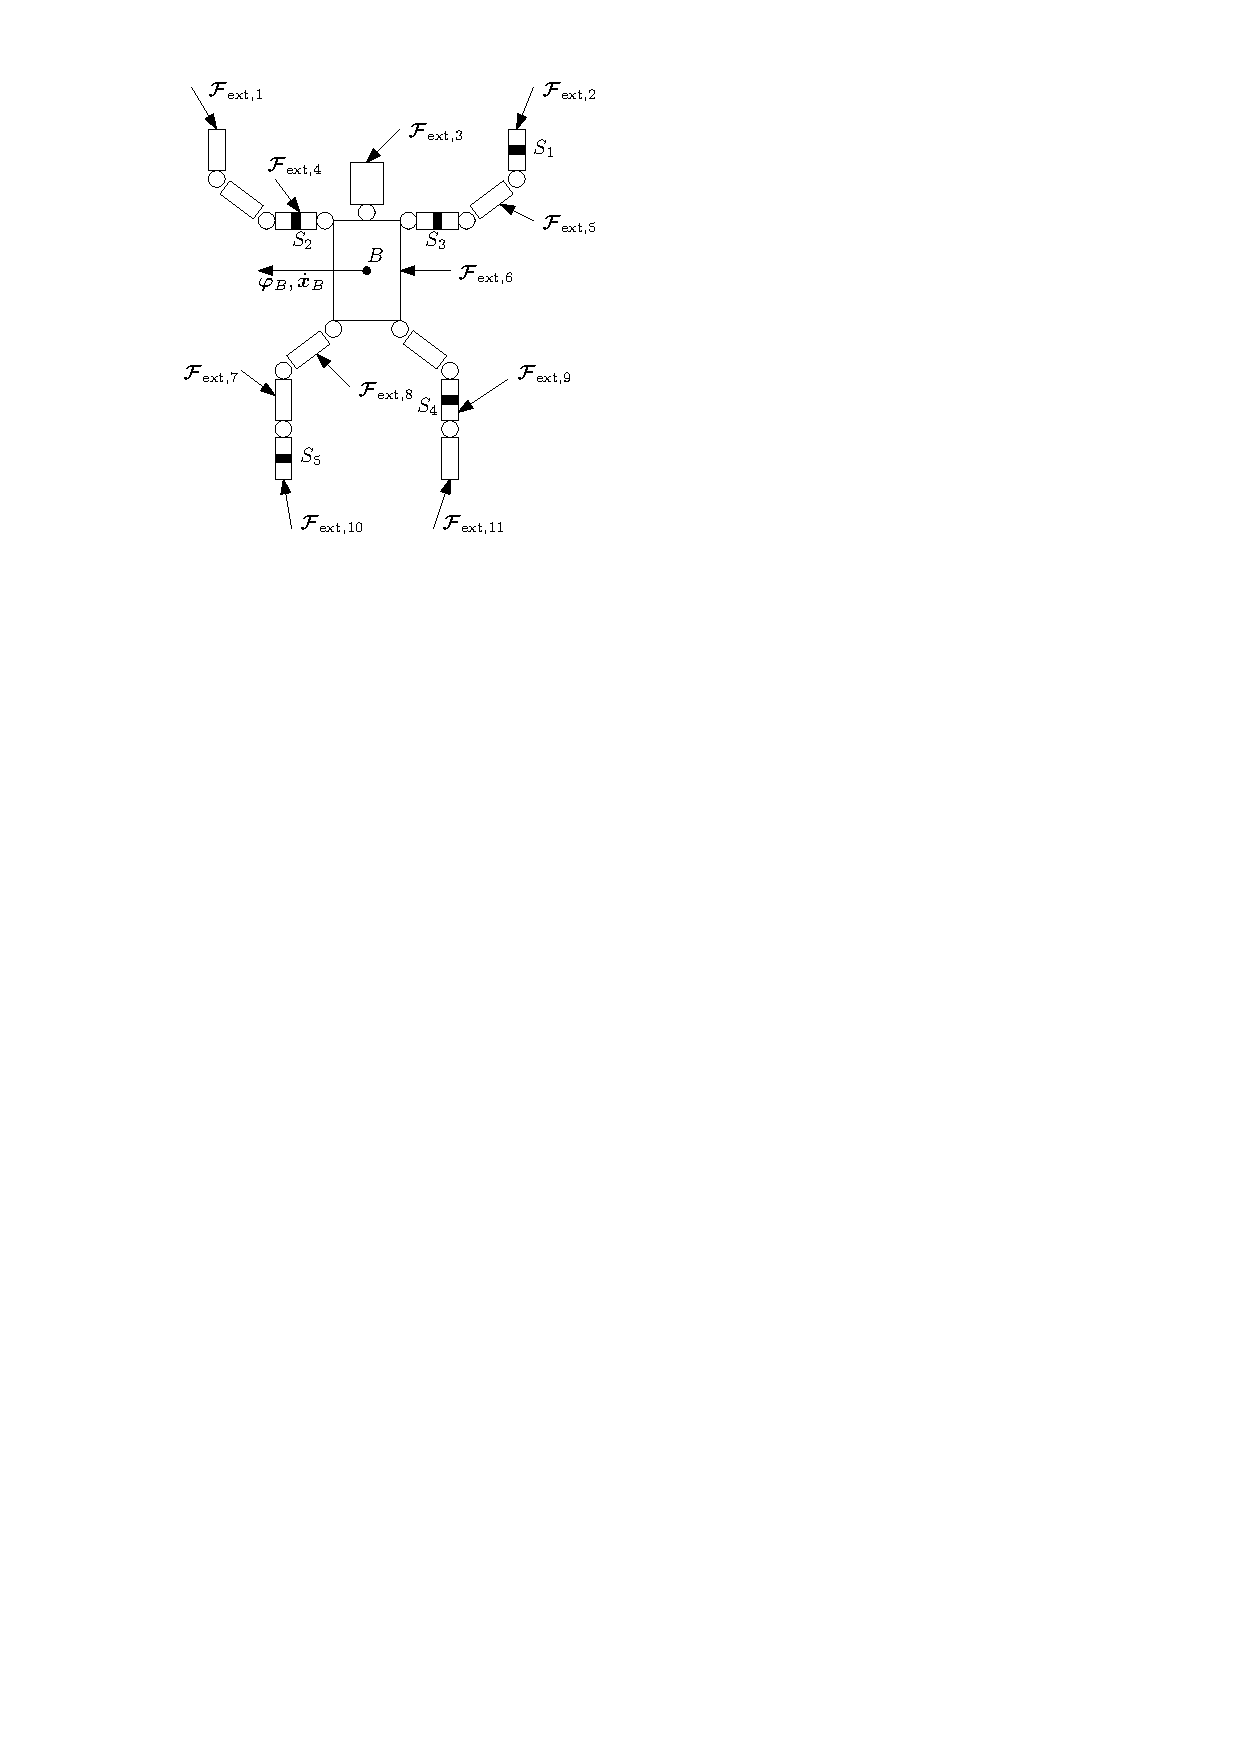
\includegraphics{figures/humanoid_contact_situation}
\end{center}
\caption{Considered problem of a humanoid robot in multiple contact situation.
External wrenches $\bm{\mathcal{F}}_{\mathrm{ext},k}$ are acting anywhere along its structure.
Forces in the feet originate from locomotion, forces at the hands may originate from manipulation.
Other external forces are caused by possibly unwanted collisions.
Also a number of force/torque sensors $S_l$ (5 in this concrete example) are distributed arbitrarily along the robot structure.}\vspace*{-0.7cm}
\label{fig:humanoid_contact_situation}
\end{figure}

Table~\ref{tab:sensors} lists the measurement quantities required to solve the problem and provides examples of suitable sensors.
Note that joint acceleration is typically not measured.
Furthermore, common acceleration sensors usually suffer from drift.
%
\begin{table}
\vspace*{0.5cm}
\caption{Measured quantities and sensors for the proposed collision detection, isolation and identification algorithm.}\label{tab:sensors}
\begin{tabular}{|c|c|c|}
\hline
robot part & measurement quantity & typical sensor\\\hline
base & $\bm{\varphi}_\mathrm{B},\dot{\bm{x}}_\mathrm{B}$ & gyroscope, Kalman estimator\\
limbs & $\bm{\tau}_\mathrm{Jm},\bm{q}_\mathrm{J},\dot{\bm{q}}_\mathrm{J}$ & joint torque sensor, encoders\\
 & $\bm{\mathcal{F}}_{S}$ & force/torque sensor\\
end-effectors & $\bm{\mathcal{F}}_{S,\mathrm{distal}}$ & force/torque sensor\\\hline
\end{tabular}\vspace*{-0.7cm}
\end{table}



\section{Collision Identification -- Part I}
\label{sec:collision_identification_i}

The first step of the proposed solution is to obtain an estimate $\hat{\bm{\tau}}_\varepsilon$ of the generalized external forces $\bm{\tau}_\mathrm{ext}$ generated by all contacts.
This can be achieved with the generalized momentum observer from \cite{DeLucaMat2003,DeLucaMat2004,Haddadin2014}, which is defined as
\begin{equation}
\hat{\bm{\tau}}_\mathrm{\varepsilon}=\bm{K}_\mathrm{O}
\left(
\bm{M}(\bm{q})\dot{\bm{q}}
-\int\limits_0^t
 [\bm{\tau}_\mathrm{m}
 -\bm{\gamma}(\bm{q},\dot{\bm{q}})
 +\hat{\bm{\tau}}_\mathrm{\varepsilon}
 ]\mathrm{d}\tilde{t} 
 \right).
\label{eqn:obs_qDD}
\end{equation}
%
It generates an estimate $\hat{\bm{\tau}}_\varepsilon$ of the generalized external forces acting on the robot, where $\bm{K}_\mathrm{O}=\mathrm{diag}\{k_{\mathrm{O},i}\}>\bm{0}$ is the observer gain matrix and
\begingroup % damit spacing in align angepasst werden kann
\medmuskip=3mu
\thinmuskip=3mu
\thickmuskip=3mu
\begin{align}
\bm{\gamma}(\bm{q},\dot{\bm{q}}):=
\bm{n}(\bm{q},\dot{\bm{q}})-\dot{\bm{M}}(\bm{q})\dot{\bm{q}}
&=\bm{g}(\bm{q})
+\bm{C}(\bm{q},\dot{\bm{q}})\dot{\bm{q}}\nonumber
-\dot{\bm{M}}(\bm{q})\dot{\bm{q}}\\
&=
\bm{g}(\bm{q})-\bm{C}^\mathrm{T}(\bm{q},\dot{\bm{q}})\dot{\bm{q}}\;
\label{eqn:gamma}
\end{align}
\endgroup
%
due to the skew-symmetry of $\dot{\bm{M}}(\bm{q})-2\bm{C}(\bm{q},\dot{\bm{q}})$ \cite{DeLucaAlbHadHir2006}.
Under ideal conditions, which means that $\bm{q}, \dot{\bm{q}}, \bm{M}(\bm{q}), \bm{C}(\bm{q},\dot{\bm{q}}), \bm{g}(\bm{q})$ are known exactly, the observer dynamics are decoupled and every component $\hat{\bm{\tau}}_{\varepsilon}$ follows the first order dynamics
%
\begin{equation}
\bm{K}_\mathrm{O}^{-1}\hat{\dot{\bm{\tau}}}_{\varepsilon}+\hat{\bm{\tau}}_{\varepsilon}=\bm{\tau}_{\mathrm{ext}}\;.\label{eqn:obs_dynamic}
\end{equation}
%
Therefore, $\hat{\bm{\tau}}_{\varepsilon}$ is simply a first order filtered version of $\bm{\tau}_{\mathrm{ext}}$.

\subsection{Estimating Generalized Acceleration}

In order to be able to determine as many contact wrenches and locations as possible, the external torques already isolated and identified by force/torque sensors are to be excluded from the observed generalized external forces $\hat{\bm{\tau}}_\varepsilon$ \cite{VorndammeSchToeHad2016}.
Therefore, we need to compensate for the dynamic and static forces generated by the mass/inertia attached to each sensor.
For this compensation, the acceleration in Cartesian space $\ddot{\bm{x}}_D$ of its center of mass $D$ is required.
Assuming the sensor $S$ to be mounted on link $i$, it may simply be calculated via
%
\begin{equation}
\ddot{\bm{x}}_D=\begin{pmatrix}
\ddot{\bm{r}}_D\\\dot{\bm{\omega}}_D
\end{pmatrix}=\bm{J}(D,i)\ddot{\bm{q}}+\dot{\bm{J}}(D,i)\dot{\bm{q}}\;.
\label{eqn:accel_cart}
\end{equation}
%
As one can see, the generalized acceleration $\ddot{\bm{q}}$ is needed to calculate the Cartesian acceleration.
An estimate $\hat{\ddot{\bm{q}}}$ of $\ddot{\bm{q}}$ can be obtained from extending the disturbance observer (\ref{eqn:obs_qDD}).
Using its inner state
%
\begin{equation}
\hat{\dot{\bm{p}}}=\bm{M}(\bm{q})\hat{\ddot{\bm{q}}}+\dot{\bm{M}}(\bm{q})\dot{\bm{q}}=\bm{\tau}_\mathrm{m}
 -\bm{\gamma}(\bm{q},\dot{\bm{q}})
 +\hat{\bm{\tau}}_\mathrm{\varepsilon}\label{eqn:impulseD}
\end{equation}
%
the estimated acceleration follows as
%
\begin{equation}
\hat{\ddot{\bm{q}}}=\bm{M}(\bm{q})^{-1}(\hat{\dot{\bm{p}}}-\dot{\bm{M}}(\bm{q})\dot{\bm{q}})=
\bm{M}(\bm{q})^{-1}(\bm{\tau}_\mathrm{m}-\bm{n}(\bm{q},\dot{\bm{q}})+\hat{\bm{\tau}}_\mathrm{\varepsilon})\;.
\end{equation}
%
The dynamics of the acceleration error $\bm{e}:=\ddot{\bm{q}}-\hat{\ddot{\bm{q}}}$ can be derived using~(\ref{eqn:impulseD}):
%
\begin{align}
\bm{e}&=\bm{M}(\bm{q})^{-1}(\dot{\bm{p}}-\dot{\bm{M}}(\bm{q})\dot{\bm{q}})-\bm{M}(\bm{q})^{-1}(\hat{\dot{\bm{p}}}-\dot{\bm{M}}(\bm{q})\dot{\bm{q}})\nonumber\\
&=\bm{M}(\bm{q})^{-1}(\bm{\tau}_\mathrm{m}-\bm{n}(\bm{q},\dot{\bm{q}})+\bm{\tau}_\mathrm{\mathrm{ext}}-(\bm{\tau}_\mathrm{m}-\bm{n}(\bm{q},\dot{\bm{q}})+\hat{\bm{\tau}}_\mathrm{\varepsilon}))\nonumber\\
&=\bm{M}(\bm{q})^{-1}(\bm{\tau}_\mathrm{\mathrm{ext}}-\hat{\bm{\tau}}_\mathrm{\varepsilon})\;.\label{eqn:qDD_dyn}
\end{align}
%
Using the Laplace transform on~(\ref{eqn:obs_dynamic}) and~(\ref{eqn:qDD_dyn}) and assuming $\bm{M}(\bm{q})$ to change slowly, we achieve the following dynamics:
%
\begin{equation}
%\bm{M}(\bm{q})^{-1}\left(\begin{pmatrix}\frac{\tau_{\mathrm{ext},1}}{1+sK_{O,1}^{-1}}\\\vdots\\\frac{\tau_{\mathrm{ext},n}}{1+sK_{O,n}^{-1}}\end{pmatrix}-\bm{\tau}_\mathrm{ext}\right)
\bm{e}=\bm{M}(\bm{q})^{-1}\begin{pmatrix}\frac{sk_{\mathrm{O},1}^{-1}\tau_{\mathrm{ext},1}}{1+sk_{\mathrm{O},1}^{-1}} &\dots&\frac{sk_{\mathrm{O},n}^{-1}\tau_{\mathrm{ext},n}}{1+sk_{\mathrm{O},n}^{-1}}\end{pmatrix}^\mathrm{T}\hspace*{-2mm}.\label{eqn:acc_err_dyn}
\end{equation}
%
The error dynamics (\ref{eqn:acc_err_dyn}) consist of a vector with a linear dynamics triggered by $\bm{\tau}_\mathrm{ext}$, which is coupled nonlinearly by the inverted mass matrix to the error $\bm{e}$.
The estimate $\hat{\ddot{\bm{q}}}$ can be used to calculate $\ddot{\bm{x}}_D$ according to (\ref{eqn:accel_cart}) and therefore the external wrench $\bm{\mathcal{F}}_{\mathrm{ext}}$, as shown next.

\subsection{Dynamic Load Compensation}
\label{sec:load_comp}

\paragraph{Distal Sensor Case}
Figure~\ref{fig:fkb} depicts the free body diagram of a distal link containing a force/torque sensor $S$ measuring a wrench $\bm{\mathcal{F}}_S$.
The left part belongs to the link connected to the base holding the sensor.
The right part represents the body attached to the sensor generating gravitational and dynamic forces measured in the sensor.
The body mass is $m_D$ and its inertia tensor $\bm{I}_{D}$.
%
\begin{figure}
\begin{center}
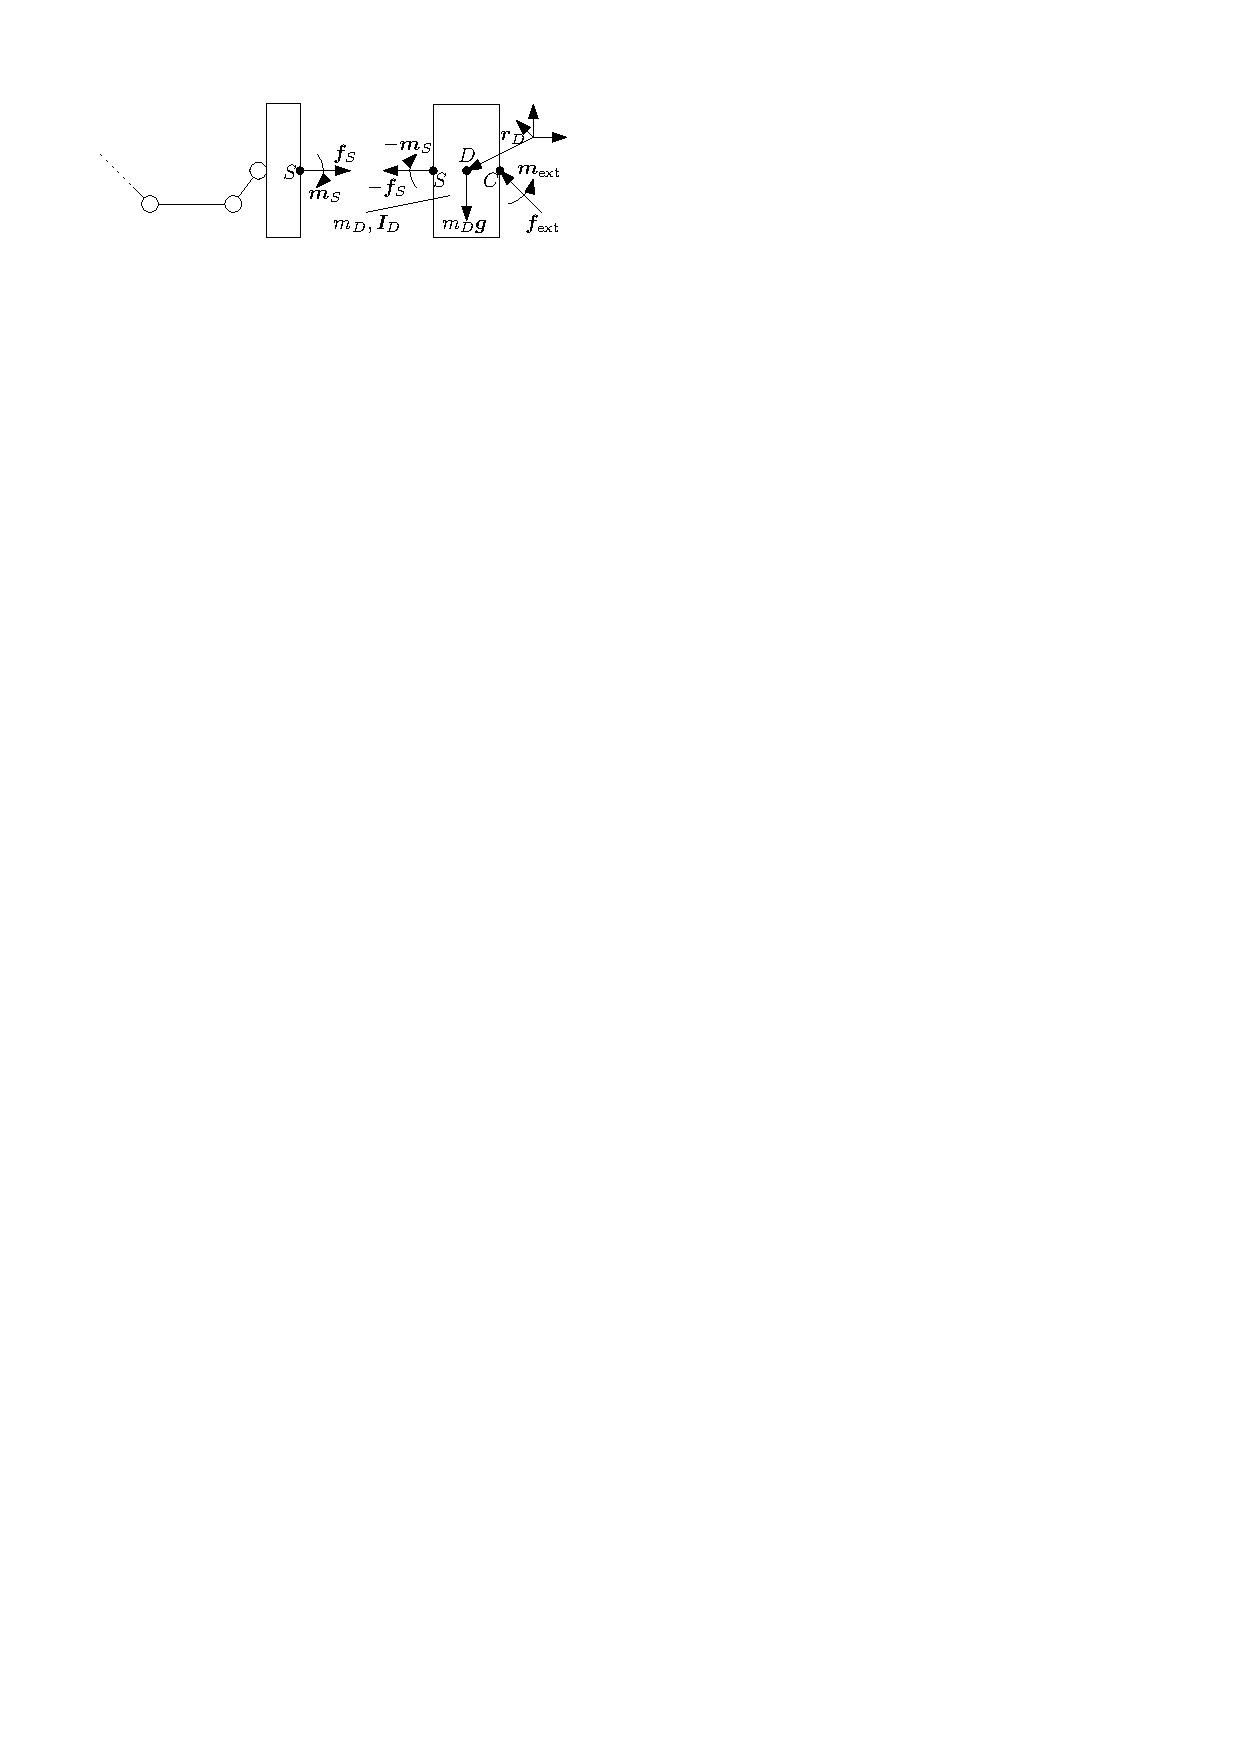
\includegraphics{figures/freikoerperbild}
\end{center}
\caption{Free body diagram of a distal robot link containing a sensor $S$.
The sensor holds a body with mass $m_D$, center of mass $D$ and inertia $\bm{I}_\mathrm{D}$.
An external force $\bm{f}_\mathrm{ext}$ and an external moment $\bm{m}_{\mathrm{ext},C}$ act in contact point $C$.}\vspace*{-0.7cm}
\label{fig:fkb}
\end{figure}
%
Newton's second law yields
\begin{equation}
m_D\ddot{\bm{r}}_D=m_D\bm{g}+\bm{f}_\mathrm{ext}-\bm{f}_S\;.
\end{equation}
%
It follows for the \textbf{sensed} external force
%
\begin{equation}
\bar{\bm{f}}_{\mathrm{ext},S}=\bm{f}_S+m_D\ddot{\bm{r}}_D-m_D\bm{g}\;.\label{eqn:fbs}
\end{equation}
%
Obviously, equation~(\ref{eqn:fbs}) shows that the sensor does not measure the pure external forces only, but also forces due to gravity and inertia.
Thus, $\bm{\mathcal{F}}_S$ has to be corrected in order to obtain the true external wrench.

To derive the external moment, Euler's law of rigid body motion is applied to the center of gravity $D$ of the body:
%
\begin{equation}%\small
\medmuskip=0mu
\thinmuskip=0mu
\thickmuskip=0mu
\bm{I}_{D}\dot{\bm{\omega}}_D+\bm{\omega}_D\times \bm{I}_{D}\bm{\omega}_D=\bm{m}_{\mathrm{ext}}-\bm{m}_S-\bm{r}_{DS}\times\bm{f}_S+\bm{r}_{DC}\times\bm{f}_\mathrm{ext}\;.\label{eqn:mbs}
\end{equation}
%
This leads to the \textbf{sensed} external moment
%
\begingroup
\small
\begin{align}
\bar{\bm{m}}_{\mathrm{ext},S}:&=
\bm{m}_{\mathrm{ext}}+\bm{r}_{SC}\times\bm{f}_\mathrm{ext}\nonumber\\&=
\bm{m}_S+\bm{I}_{D}\dot{\bm{\omega}}_D+\bm{\omega}_D\times \bm{I}_{D}\bm{\omega}_D+\bm{r}_{DS}\times(\bm{f}_S-\bm{f}_\mathrm{ext})\;.
\end{align}
\endgroup
%
Equations~(\ref{eqn:fbs}) and~(\ref{eqn:mbs}) result in the \textbf{sensed} external wrench 
%
\begingroup % damit spacing in align angepasst werden kann
\medmuskip=2mu
\thinmuskip=2mu
\thickmuskip=2mu
\small
\begin{align}
\bar{\bm{\mathcal{F}}}_{\mathrm{ext},S}&=\begin{pmatrix}
\bar{\bm{f}}_{\mathrm{ext},S}\\\bar{\bm{m}}_{\mathrm{ext},S}\nonumber
\end{pmatrix}=\bm{\mathcal{F}}_{S}+\bm{\mathcal{F}}_{c,S}\\
:&=\bm{\mathcal{F}}_S+\left(\begin{smallmatrix}
m_D\bm{I}_3 & \bm{0}\\
m_D\bm{S}(\bm{r}_{SD}) & \bm{I}_{D}
\end{smallmatrix}\right)
\left(\left(\begin{smallmatrix}\ddot{\bm{r}}_D\\\dot{\bm{\omega}}_D\end{smallmatrix}\right)-\left(\begin{smallmatrix}
\bm{g}\\\bm{0}
\end{smallmatrix}\right)\right)+\left(\begin{smallmatrix}
\bm{0}\\
\bm{\omega}_D\times\bm{I}_{D}\bm{\omega}_D
\end{smallmatrix}\right).\label{eqn:ext_wrench}
\end{align}
\endgroup
%
$\bm{I}_3$ denotes the three dimensional unit matrix, $\bm{g}$ the Cartesian gravity vector, $\bm{r}_{DS}$ the vector from the center of mass of the inertia attached to the sensor to the sensor and $\bm{0}$ the zero matrix of suitable size.
All entities are expressed in the world frame.
Using $\hat{\ddot{\bm{q}}}$ instead of $\ddot{\bm{q}}$ in~(\ref{eqn:accel_cart}) to compute $\hat{\ddot{\bm{x}}}_D$ one obtains the estimated external wrench acting in $S$ as
%
\begin{equation}\small
\medmuskip=2mu
\thinmuskip=2mu
\thickmuskip=2mu
\hat{\bm{\mathcal{F}}}_{\mathrm{ext},S}=\bm{\mathcal{F}}_S+\underbrace{\left(\begin{smallmatrix}
m_D\bm{I}_3 & \bm{0}\\
m_D\bm{S}(\bm{r}_{SD}) & \bm{I}_{D}
\end{smallmatrix}\right)
\left(\left(\begin{smallmatrix}\hat{\ddot{\bm{r}}}_D\\\hat{\dot{\bm{\omega}}}_D\end{smallmatrix}\right)-\left(\begin{smallmatrix}
\bm{g}\\\bm{0}
\end{smallmatrix}\right)\right)+\left(\begin{smallmatrix}
\bm{0}\\
\bm{\omega}_D\times\bm{I}_\mathrm{D}\bm{\omega}_D
\end{smallmatrix}\right)}_{\hat{\bm{\mathcal{F}}}_{c,S}}\;.
\end{equation}
 
\paragraph{Intermediate Sensor Case}
If the sensor is located within an intermediate link, the compensation wrenches for each body $b$, with center of mass $D_b$, succeeding this sensor become
%
\begin{equation}
\medmuskip=0mu
\thinmuskip=0mu
\thickmuskip=0mu
\small
\hat{\bm{\mathcal{F}}}_{\mathrm{c},b}=\left(\begin{smallmatrix}
m_{D_b}\bm{I}_3 & \bm{0}\\
m_{D_b}\bm{S}(\bm{r}_{SD_b}) & \bm{I}_{D_b}
\end{smallmatrix}\right)
\left(\left(\begin{smallmatrix}\hat{\ddot{\bm{r}}}_{D_b}\\\hat{\dot{\bm{\omega}}}_{D_b}\end{smallmatrix}\right)-\left(\begin{smallmatrix}
\bm{g}\\\bm{0}
\end{smallmatrix}\right)\right)+\left(\begin{smallmatrix}
\bm{0}\\
\bm{\omega}_{D_b}\times\bm{I}_{D_b}\bm{\omega}_{D_b}
\end{smallmatrix}\right)
\end{equation}
%
and simply have to be summed up for compensation.
Note that this operation explicitly corresponds to the Newton- Euler method for calculating multibody dynamics.
Therefore, in this case, the estimated external wrench sensed in $S$ becomes
%
\begin{equation}
\hat{\bm{\mathcal{F}}}_{\mathrm{ext},S}=\bm{\mathcal{F}}_S+\sum_{b\in N(b_\mathrm{s})}\hat{\bm{\mathcal{F}}}_{\mathrm{c},b}=:\bm{\mathcal{F}}_S+\hat{\bm{\mathcal{F}}}_{\mathrm{c},S}\;.\label{eqn:cmp}
\end{equation}
%
$N(b_\mathrm{s})$ denotes the set of all bodies succeeding link $b_\mathrm{s}$, that contains the sensor in the kinematic chain.
For multiple sensors in a kinematic chain (e.g. in each joint), the compensation wrenches can be calculated recursively to avoid multiple calculations, see Algorithm~\ref{alg:comp}.
The code uses the set $M(S)$, denoting all sensors $T\in M(S)$ directly succeeding $S$.
This means there is no further sensor between $S$ and an element of $M(S)$ in the kinematic chain connecting the two.
%
\begin{algorithm}
\caption{Dynamic load compensation for multiple force/torque sensors located along the structure}
\textbf{function} $\hat{\bm{\mathcal{F}}}_{\mathrm{c},S} =$ calculate\_F\_c($S$)\\
\Begin{
	$\hat{\bm{\mathcal{F}}}_{\mathrm{c},S}:=0$\\
	\For {all bodies $b$ directly succeeding $S$}{
			$\hat{\ddot{\bm{x}}}_{D_b}=\bm{J}_{D_b}\hat{\ddot{\bm{q}}}+\dot{\bm{J}}_{D_b}\dot{\bm{q}}$\\
			$\small\hat{\bm{\mathcal{F}}}_{\mathrm{c},S}+=\left(\begin{smallmatrix}
			m_{D_b}\bm{I}_3 & \bm{0}\\
			m_{D_b}\bm{S}(\bm{r}_{SD_b}) & \bm{I}_{D_b}
			\end{smallmatrix}\right)
			\left(\hat{\ddot{\bm{x}}}_{D_b}-\left(\begin{smallmatrix}
			\bm{g}\\\bm{0}
			\end{smallmatrix}\right)\right)$\\
			$\quad\quad\quad\quad\quad+\left(\begin{smallmatrix}
			\bm{0}\\
			\bm{\omega}_{D_b}\times\bm{I}_{D_b}\bm{\omega}_{D_b}
			\end{smallmatrix}\right)$
	}
	\For {all $T\in M(S)$}{
			$\hat{\bm{\mathcal{F}}}_{\mathrm{c},T} =$ calculate\_F\_c($T$)\\
			$\hat{\bm{\mathcal{F}}}_{\mathrm{c},S}+=\hat{\bm{\mathcal{F}}}_{\mathrm{c},T}+
			\begin{pmatrix}
			\bm{0}\\\bm{r}_{ST}\times\hat{\bm{f}}_{\mathrm{ext},T}
			\end{pmatrix}$
	}
}
\label{alg:comp}
\end{algorithm}

\subsection{Generalized Contact Force Estimation}

It is to be considered for the estimation of the contact wrenches and also for the collision detection that the observer detects generalized external forces originating from all external contacts.
In particular with a humanoid, we usually have desired contacts (e.g. at the feet during locomotion or hands during manipulation), these contact forces have to be measured with force/torque sensors close to the corresponding end-effectors (e.g. at the wrists and ankles) in order to enable exclusion from the observed generalized forces and avoid undesired collision detections (``false alarms'').

The full scheme consisting of observer and compensation is depicted in Fig.~\ref{fig:flowchart}.
For sake of simplicity force/torque sensors in all distal links of the arms and legs are assumed, denoted by the set $S_\mathrm{distal}$.
The more general case, where one or more distal links do not have a force/torque sensor will be left for future work at this point.
The general consequence of such a setup would be a limited ability to detect, isolate and identify collisions occurring between the end-effector and the most distal force/torque sensor in the kinematic chain.
%
\begin{figure}
\begin{center}
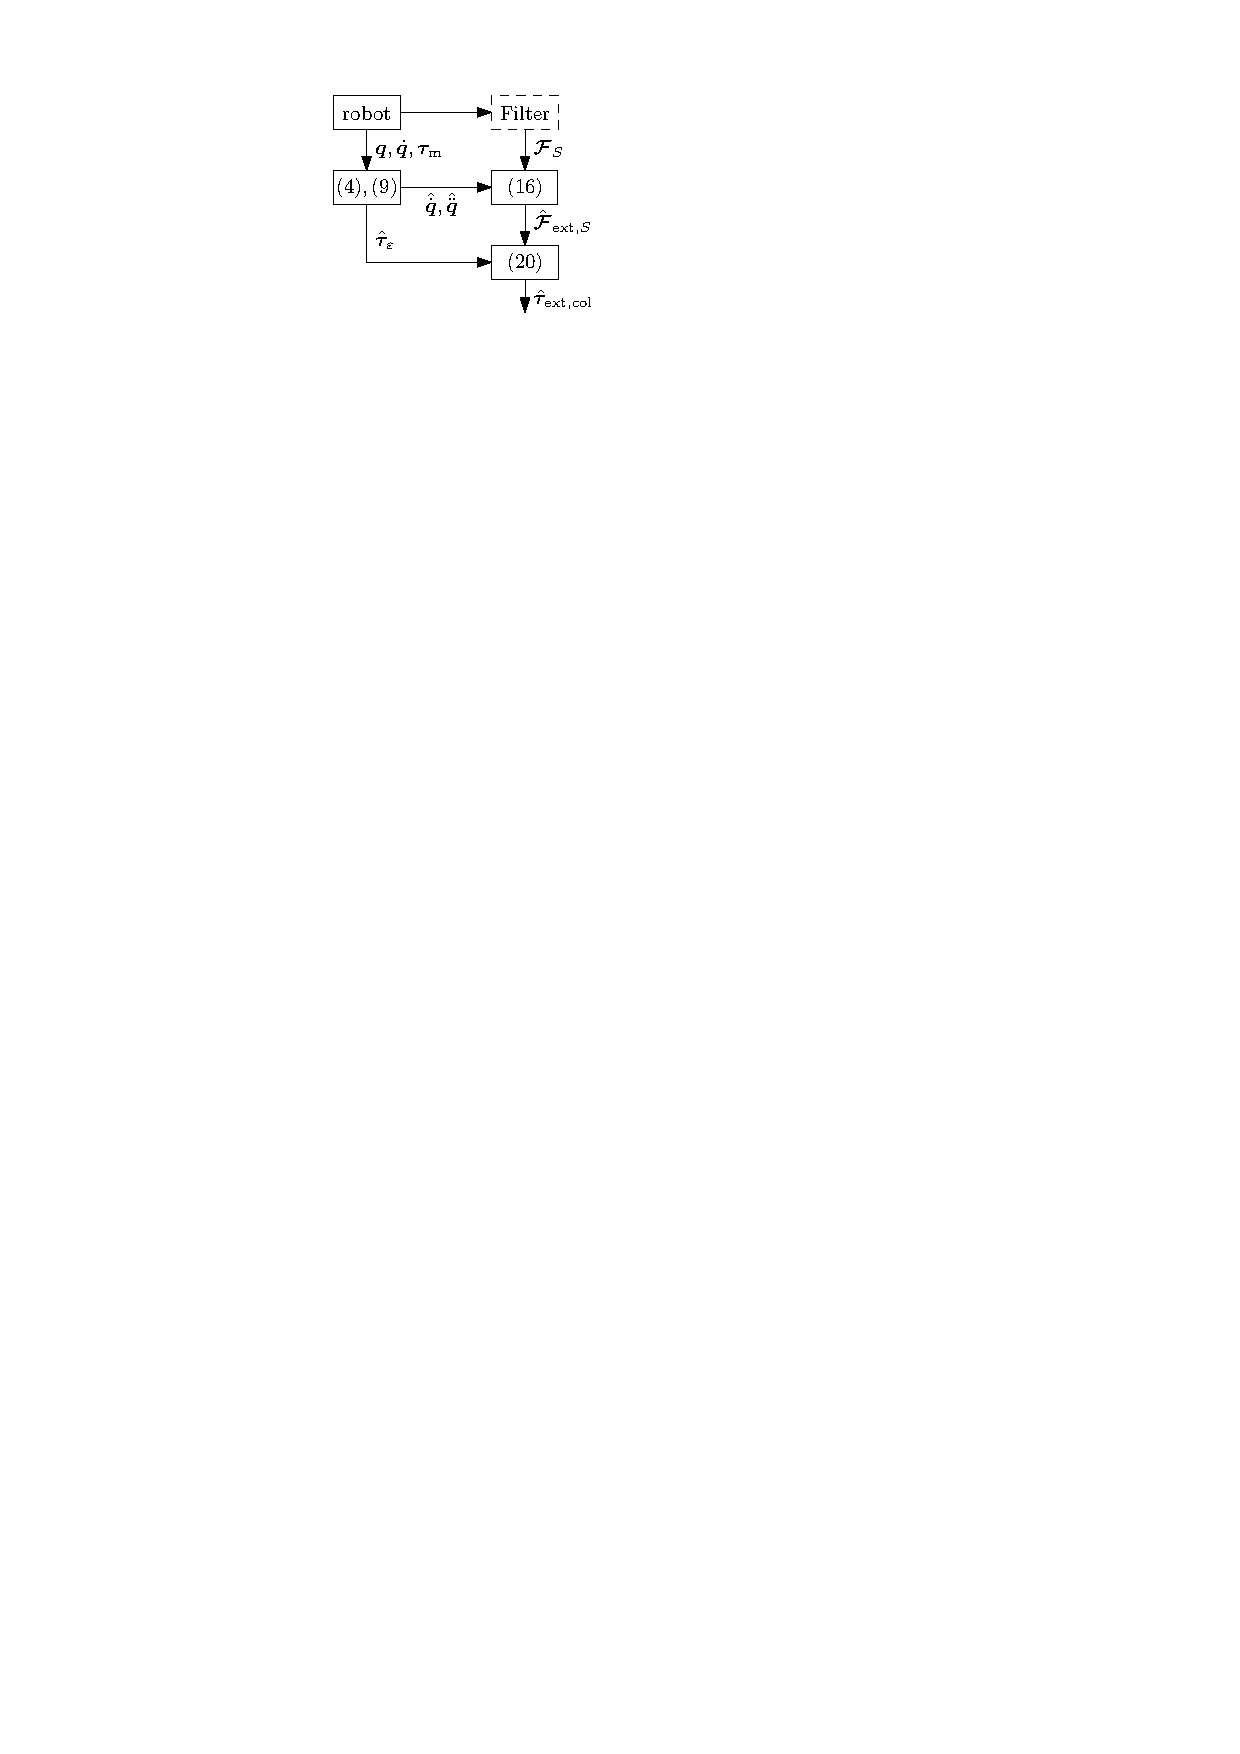
\includegraphics{figures/flowchart_compensation}
\end{center}
\caption{Exclusion of estimated desired external wrenches at the distal links $\hat{\bm{\mathcal{F}}}_{\mathrm{ext},S}$ measured by force/torque sensors from the observed generalized  forces of~(\ref{eqn:obs_qDD}).
These wrenches are therefore compensated according to~(\ref{eqn:ext_wrench}).}\vspace*{-0.8cm}
\label{fig:flowchart}
\end{figure}
%
% TODO: Keine joint forces, sondern generalized coordinates
The generalized external forces caused by the external wrenches at the distal links are subtracted from the observed generalized forces to obtain the estimated generalized forces originating from unexpected collisions $\hat{\bm{\tau}}_\mathrm{ext,col}$ as
%
\begin{equation}
\hat{\bm{\tau}}_\mathrm{ext,col}=\hat{\bm{\tau}}_\varepsilon-\sum_ {S\in S_\mathrm{distal}}\bm{J}^\mathrm{T}(S,i_S)\hat{\bm{\mathcal{F}}}_{\mathrm{ext},S}\;,\label{eqn:obs_cmp}
\end{equation}
%
where $i_S$ denotes the link containing the sensor $S$.
Now that the force/torque sensors are compensated and the desired external wrenches of the distal parts of the robot are excluded from the observed generalized external forces, collision detection can be performed.

\subsection{Collision Detection}


Collision detection is simply done via thresholding the generalized forces and estimated external wrenches
%
\begin{equation}
\begin{split}
\hat{\bm{\tau}}_\mathrm{ext,col}>\bm{\tau}_\mathrm{thresh} \text{ (element wise) or}\\
\hat{\bm{\mathcal{F}}}_{\mathrm{ext},S}>\bm{\mathcal{F}}_{S,\mathrm{thresh}} \text{ (element wise).}
\label{eqn:threshold}
\end{split}
\end{equation}
%
The information coming with evaluating (\ref{eqn:threshold}) can also be used to roughly estimate the contact location.
Contacts can always be located behind the last joint or sensor exceeding the threshold and before the next sensor not exceeding it, respectively.
To gain more precise information about the contact link, the external wrenches $\bm{\mathcal{F}}_{\mathrm{ext},k}$ are needed (see also Fig.~\ref{fig:ueberblick}).
The next section shows, how to obtain $\bm{\mathcal{F}}_{\mathrm{ext},k}$ and how to use it for collision isolation.

\section{Collision Isolation}
\label{sec:isolation}
Collision isolation cannot be generally handled for the case when external moments act along the robot. 
For this case, the contact location of an additionally acting contact force cannot be located exactly. 
Thus, for solving the isolation problem we assume no external moments to be acting on the robot ($\bm{m}_{\mathrm{ext},k}=\bm{0}$), which is a realistic assumption for most undesired collision situations.
If this assumption does not hold for a certain contact point, the isolation of this particular contact point will fail.
However, this does not influence the isolation and identification of other contact points.
In summary, isolation is done via the following four step approach:
%
\begin{enumerate}
\item Isolate the contact link,
\item estimate the external wrench acting on the respective contact link,
\item calculate the line of action of the force estimated and
\item determine the exact contact point by intersecting the line of action with the known robot geometry.
\end{enumerate}
%
For steps 2 and 3 two main scenarios have to be distinguished: single contact and multi contact scenarios.
The single contact scenario can be handled with joint torque sensing only, while the multi contact scenario often requires additional force/torque sensors in order to distinguish the different contacts.

\subsection{Single Contact}

\paragraph{Step 1}

The contact link can be found based on the fact that a contact cannot produce torques in joints appearing behind the contact location along the kinematic chain.
E.g., a contact at the upper arm cannot produce torques in the wrist.
Therefore, the contact link index $i$ can be isolated by
%
\begin{equation}
i=\max\{j|\tau_{\mathrm{ext,col},j} \neq 0\}
\label{eqn:contact_link}
\end{equation}
%
given the convention that joint $j$ connects link $j$ to the preceding links of the robot.
Note that due to the tree structure of a humanoid, this procedure can lead to multiple potential contact links. It has to be noted also that due to modeling and measurement errors, eq.~(\ref{eqn:contact_link}) is subject to thresholding.
Also some forces, e.g. forces parallel to the axis of the joint connected to the link they act on, do not produce torques at this joint. This may lead to erroneous estimation of the contact link. However, this problem can be tackled with a correction step introduced at the end of step~4.

\paragraph{Step 2}

When the contact link $i$ with origin $O_i$ is found, the external wrench $\bm{\mathcal{F}}_i$ acting on this respective link may be estimated via the Moore-Penrose pseudo inverse of $\bm{J}^\mathrm{T}(O_i,i)$:
%
\begin{equation}
\hat{\bm{\mathcal{F}}}_i=(\bm{J}^\mathrm{T}(O_i,i))^\#\hat{\bm{\tau}}_\mathrm{ext,col}\;.\label{eqn:F_i}
\end{equation}
%
\paragraph{Step 3}
\label{sec:isolation_step3}
For a single external wrench $\bm{\mathcal{F}}_\mathrm{ext}$ acting at the contact location $\bm{r}_C$, the wrench $\bm{\mathcal{F}}_i$ in $O_i$ may be obtained with the adjoint matrix $\bm{A}(C,O_i)$ via
%
\begin{equation}
\bm{\mathcal{F}}_i=\bm{A}^\mathrm{T}(C,O_i)\bm{\mathcal{F}}_\mathrm{ext}
=\begin{pmatrix} \bm{I}_3 & \bm{0}\\
\bm{S}(\bm{r}_{O_iC}) & \bm{I}_3\end{pmatrix}
\bm{\mathcal{F}}_\mathrm{ext}\;.\label{eqn:ext_wrench_i}
\end{equation}
%
Recalling the assumption of absence of external moments ($\bm{m}_\mathrm{ext}=\bm{0}$) this results in
%
\begin{equation}
\bm{\mathcal{F}}_i=\begin{pmatrix} \bm{f}_i\\\bm{m}_i\end{pmatrix}
=\begin{pmatrix}
\bm{f}_\mathrm{ext}\\\bm{S}(\bm{r}_{O_iC})\bm{f}_\mathrm{ext}
\end{pmatrix}=\begin{pmatrix}
\bm{f}_i\\\bm{S}^\mathrm{T}(\bm{f}_i)\bm{r}_{O_iC}
\end{pmatrix}.\label{eqn:contact_pkt}
\end{equation}
%
From~(\ref{eqn:contact_pkt}), the line of action of the force can be derived.
It is described by $\bm{r}_{A}+\lambda\bm{f}_i/\|\bm{f}_i\|$ for $\lambda\in\mathbb{R}$ with
%
\begin{equation}
\bm{r}_A=\bm{r}_{O_i}+\bm{r}_{O_iA}=\bm{r}_{O_i}+\left(\bm{S}^\mathrm{T}(\bm{f}_i)\right)^\#\bm{m}_i\;.
\label{equ:force_loa_point}
\end{equation}
%

\paragraph{Step 4}
\label{sec:isolation_step4}
Due to the properties of the pseudo inverse and the rank deficit of skew symmetric matrices, $\bm{r}_{A}$ is the point along the line of action of the force, which lies closest to the origin and therefore is not identical to $\bm{r}_C$ in general.
However, it is possible to calculate $\bm{r}_C$ by intersecting the line of action of the force with the link geometry of the contact link.
If this intersection problem has more than one solution, the one with the smallest parameter $\lambda$ can e.g. be chosen.
This choice is made when we assume a pushing force, which is most common for unexpected collisions.
However, all candidates can be generated and utilized if more sophisticated processing is done at a higher level of abstraction.

If the contact link is not estimated correctly, the contact point $\bm{r}_C$ can nonetheless be computed for the single contact case, as the base movement provides sufficient information to determine it.
This happens e.g. if the contact force is parallel to the axis of the joint connected to the link it is acting on or line of action of the force crosses this joint axis.
In this case, the line of action may happen to not intersect the estimated contact link.
Therefore, the contact point $\bm{r}_C$ may be determined correctly by intersecting the line of action also with the subsequent links.

\subsection{Multiple Contacts}

For the case of multiple contacts, above method may be used in combination with compensated force/torque sensing. Then, for each sensor, a contact in the kinematic chain following the sensor may be detected by applying steps 3 and 4 for the compensated (in the sense of~(\ref{eqn:ext_wrench})~or~(\ref{eqn:cmp})) wrenches $\hat{\bm{\mathcal{F}}}_{\mathrm{ext},S}$ of the sensors.
In case of more than one sensor and more than one contact in the kinematic chain, the wrenches originating from contacts already measured by sensors closer to the distal end of the chain have to be subtracted from the measured wrench.
As a sensor sees all contact wrenches acting on subsequent sensors with an additional moment because of the change in lever of the force, in addition to the external wrenches exclusively seen by it, this leads to
%
\begin{equation}
\hat{\bm{\mathcal{F}}}_{\mathrm{ext},k}=\hat{\bm{\mathcal{F}}}_{\mathrm{ext},S}-\sum_{T\in N(S)}\left(\hat{\bm{\mathcal{F}}}_{\mathrm{ext},T}+\begin{pmatrix}
\bm{0}\\\bm{r}_{ST}\times\hat{\bm{f}}_{\mathrm{ext},T}
\end{pmatrix}\right).\label{eqn:cmp_ext_vorher}
\end{equation}
%
Considering the situation of Fig.~\ref{fig:humanoid_contact_situation} for example, two contacts can be detected at the right arm.
One by sensor $S_3$ and one by sensor $S_1$, as long as one contact is behind $S_1$ and the other between $S_3$ and $S_1$.
As this is the case for $\bm{\mathcal{F}}_{\mathrm{ext},2}$ and $\bm{\mathcal{F}}_{\mathrm{ext},5}$ these two wrenches may be estimated correctly.

If no force/torque sensors are available the correct isolation of multiple contacts is only possible if the contact links are estimated correctly and are far enough away from the base, which means that the Jacobians of the contact links together include at least 6~DOFs per wrench to estimate. For this, the contact wrenches may be calculated by stacking the Jacobians together and calculating the according pseudoinverse
%
\begin{equation}
\medmuskip=3mu
\thinmuskip=3mu
\thickmuskip=3mu
\left(
\bm{\mathcal{F}}_{i_1}^\mathrm{T} \ldots \bm{\mathcal{F}}_{i_n}^\mathrm{T}\right)^\mathrm{T}=\left(
\bm{J}^\mathrm{T}(O_{i_1},i_1) \ldots  \bm{J}^\mathrm{T}(O_{i_n},i_n)\right)^\#\bm{\tau}_\mathrm{ext,col}\;.\label{eqn:multi_iso}
\end{equation}
%
Note that in case of a singularity in the Jacobians additional DOFs may be required to estimate the wrenches correctly.
Thereafter, steps 3 and 4 can be applied to each estimated wrench $\bm{\mathcal{F}}_{i}$. This step may be considered  a generalization of eq. (6) in \cite{OttHenLee2013}.

\section{Collision Identification -- Part II}

Now that the contact points are determined, the full contact Jacobians
%
\begin{equation}
\bm{J}(C,i)=\bm{A}(C,O_i)\bm{J}(O_i,i)
\end{equation}
%
may be computed.
Similar to~(\ref{eqn:multi_iso}) they can be used to identify the external wrenches
%
\begin{equation}
\medmuskip=1mu
\thinmuskip=1mu
\thickmuskip=1mu
\left(
\bm{\mathcal{F}}_\mathrm{ext,1}^\mathrm{T} \ldots \bm{\mathcal{F}}_{\mathrm{ext},n}^\mathrm{T}\right)^\mathrm{T}=\left(
\bm{J}^\mathrm{T}(C_1,i_1) \ldots \bm{J}^\mathrm{T}(C_n,i_n)\right)^\#\bm{\tau}_\mathrm{ext,col}\;.
\label{eqn:force_identification}
\end{equation}
%
This step is only neccessary, if the contact points are found in different links than determined by (\ref{eqn:contact_link}).
In this case, measurements of additional joints are used to improve the result of (\ref{eqn:F_i}).
Otherwise, the inverse of (\ref{eqn:ext_wrench_i}) can be used directly to calculate the contact wrenches.
For wrenches identified with a force/torque sensor, no action has to be taken in this step, as the corrected wrenches are already the best estimates.
Figure~\ref{fig:ueberblick} depicts an overview of the entire algorithm.
%
\begin{figure}
\begin{center}
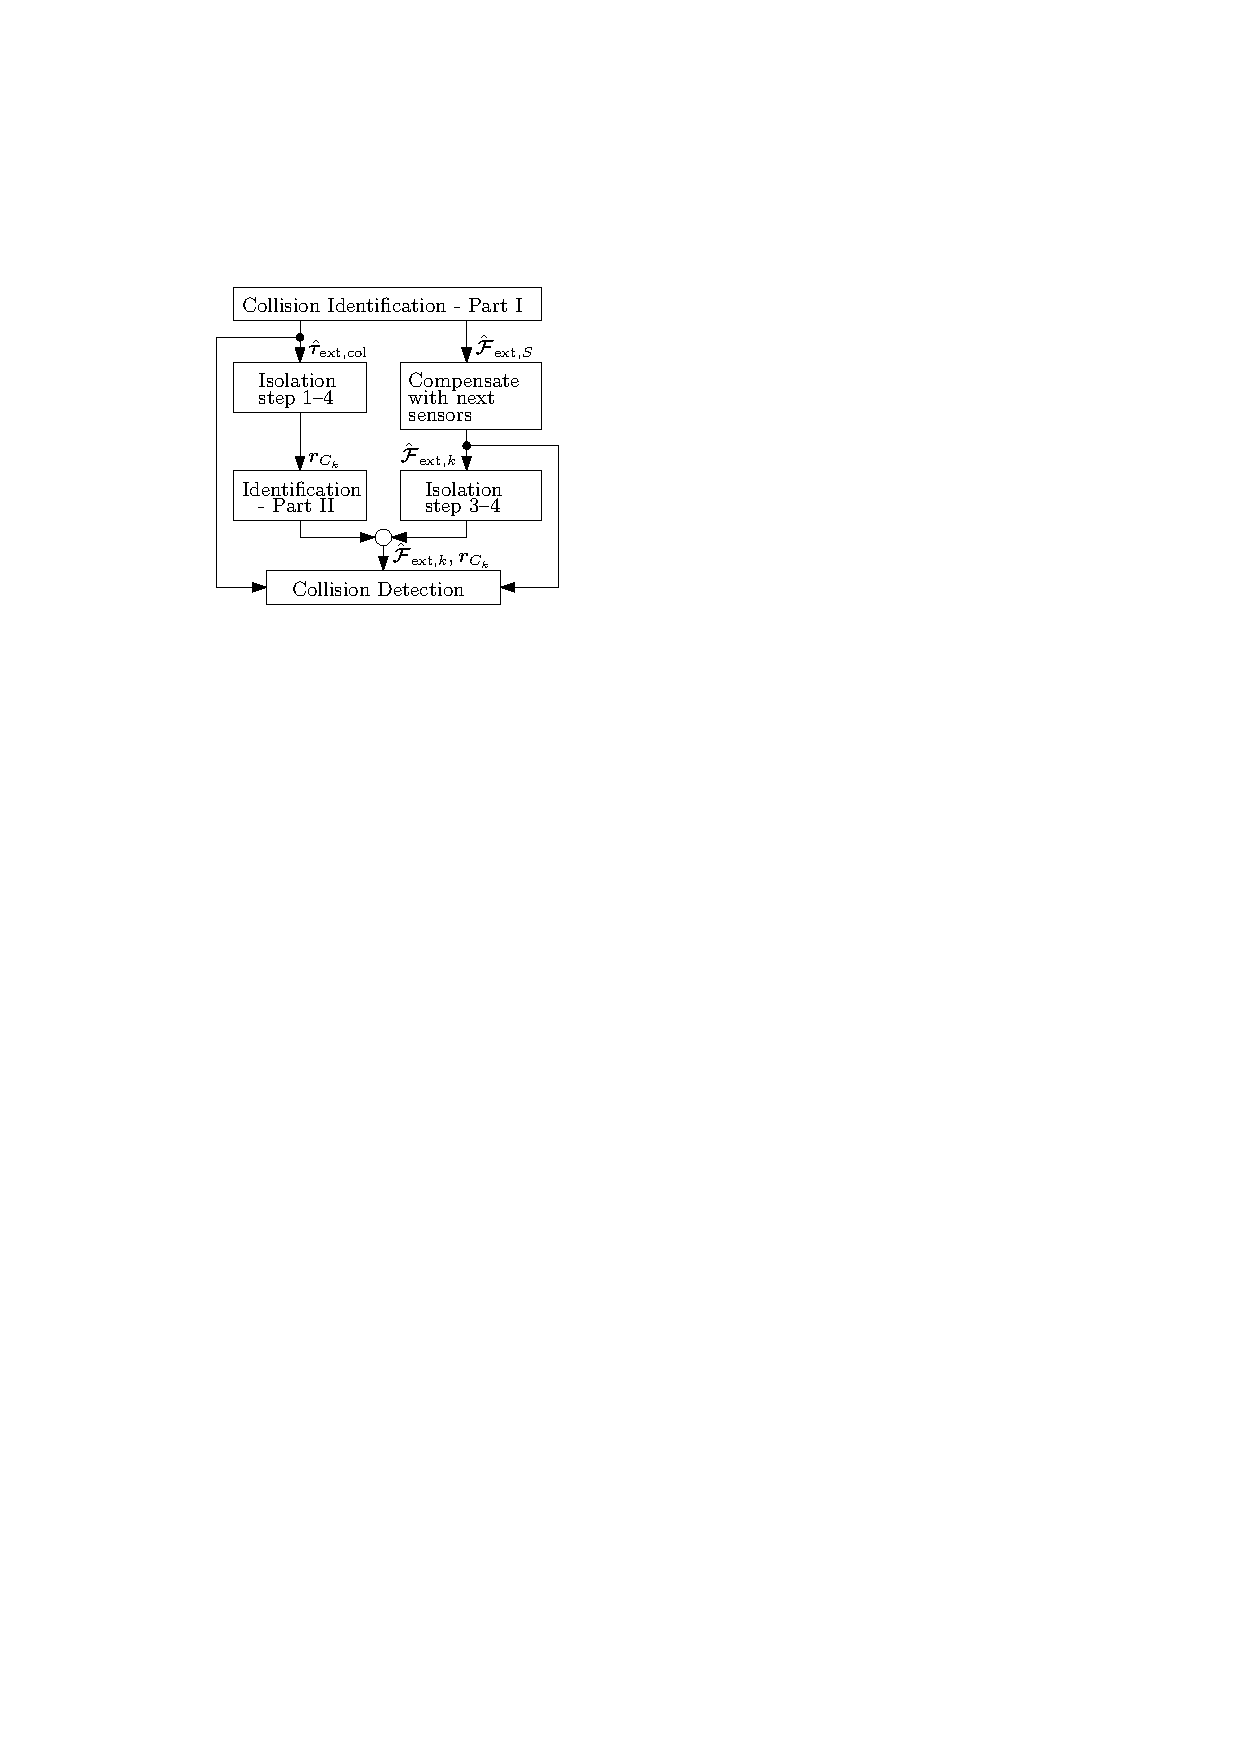
\includegraphics{figures/ueberblick}
\end{center}
\caption{An overview of the collision detection isolation and identification algorithm.
The more information is used, the more information can be obtained from the collision detection step.
If the collision detection is based on $\hat{\bm{\tau}}_\mathrm{ext,col}$ only, the contact cannot be fully located.
If $\hat{\bm{\mathcal{F}}}_{\mathrm{ext},S}$ is used in addition, the contact can be located to the parts of the robot lying between the detecting and the following sensors.
If the full $\hat{\bm{\mathcal{F}}}_{\mathrm{ext},k}$ are available, collision detection can be done on a per link basis.}\vspace*{-0.7cm}
\label{fig:ueberblick}
\end{figure}
%
In the next section, the proposed algorithm is validated in different scenarios with a simulated Atlas robot.



% !TEX root = collhdl_ICRA_17.tex

\section{Evaluation and Case Studies}
\label{sec:simu}

\subsection{General Simulation Setup}
\label{sec:setup}
The simulative setup is as follows.
We apply our collision detection, isolation and identification algorithm in simulation to an \emph{Atlas} robot consisting of cylinders and cuboids as collision geometry from \cite{DRCSim}.
We assume perfect measurements of the generalized joint forces and the force/torque sensors unless stated differently, meaning all sensors measure the true value without noise or delay.
Force/torque sensors are placed at the end-effectors (feet and hands), before the first arm and leg joints and at the upper torso after the three back joints (see Fig.~\ref{fig:coll_singlecontact_overview}).
Furthermore, all acting external forces comply with the assumption of a pushing force and the line of action of the forces is chosen such that it does not intersect with any other collision body before the contact point.
The robot pose (see Fig.~\ref{fig:coll_singlecontact_overview}) has been chosen in such a way that the whole body Jacobian has full rank.
The robot is modeled in free space, meaning there are no other external forces acting on the robot than the collision forces.
The simulation is done on a standard Core i7-3770 PC and the algorithm is run as compiled Matlab functions.
With the current implementation, the majority of the runtime for all contact cases is spent on the not yet optimized intersection algorithm.

\subsection{Ideal Analysis of Single Contacts}
\label{sec:eval_single_static}
We compare the ideal performance of the isolation based on estimated generalized external forces $\hat{\bm{\tau}}_\epsilon$ only (Sec.~\ref{sec:isolation}) to the isolation based only on force/torque sensor measurements $\hat{\bm{\mathcal{F}}}_{\mathrm{ext},S}$ (from (\ref{eqn:cmp})) for a single contact.
Dynamic effects due to the observer and load compensation are neglected for sake of clarity.
The contact points are distributed randomly and equally over the robot surface.
Figure~\ref{fig:coll_singlecontact_overview} depicts the results of the isolation procedures with some representative samples of the 3000 tested points.
With both methods, the contact points are isolated correctly up to rounding errors, if possible.
The contacts at the pelvis cannot be seen by any force/torque sensor and can therefore only be isolated with the generalized external forces acting on the base.
The maximum and mean execution times for the isolation of the one contact in this experiment were 0.67~ms and 0.25~ms using force/torque sensors as well as 0.57~ms and 0.17~ms using joint torque measurements only.
\begin{figure}
\begin{center}
\begin{overpic}{figures/collest_single_allresults_nosim/coll_est_sc_all_nosim}
\put(82,54){\line(-1,-2){7}}
\put(56,11){\line(1,2){11}}
\put(67,35){F/T sensor}
\end{overpic}
\end{center}
\caption{Distribution of true ($\bm{r}_\mathrm{C}$) and estimated contact locations using two different methods.
The points $\hat{\bm{r}}_C(\hat{\bm{\tau}}_\epsilon)$ are isolated using only generalized external forces and the points $\hat{\bm{r}}_C(\hat{\bm{\mathcal{F}}}_{\mathrm{ext,S}})$ are isolated using the force/torque sensor measurements only.
For the pelvis (base link) and first torso links, no force measurement is available. Therefore contact points at these links cannot be found with the latter method.
All overlying points are identical up to rounding errors.}
\vspace*{-0.8cm}
\label{fig:coll_singlecontact_overview}
\end{figure}

\subsection{Ideal Analysis of Multiple Contacts}
\label{sec:eval_multi_static}
In the following, we analyze multiple contacts of the type specified in Sec.~\ref{sec:eval_single_static}.

\subsubsection{Two Contacts at different links}

The considered contact points are located at different links, since two contacts at the same link cannot be located in our setup. In order to be able to do so, one would need two force/torque sensors in the same link.
5000 random combinations were examined.

The algorithm using generalized forces is able to isolate all two contact point coordinates up to rounding errors if the rank of the Jacobian in (\ref{eqn:force_identification}) is sufficiently high, e.g. $\mathrm{rank}(\bm{J})=12$ for $N_\mathrm{C}=2$ contact points.
Figure~\ref{fig:coll_multicontact_rankJ} shows the success of the isolation for different contact links, which is equivalent to the plot of the rank deficit
\begin{equation}
RD=6N_\mathrm{C}-\mathrm{rank}(\bm{J}).
\label{eqn:rank_deficit}
\end{equation}
For example, a contact at the pelvis (torso chain link 1) and another contact at the left lower leg (left leg chain link 4) does only produce 10 nonzero columns in the stacked Jacobian and the isolation fails (see corresponding entry in Fig.~\ref{fig:coll_multicontact_rankJ}).
If instead the foot on the left leg chain (link 6) is in contact, then 12 nonzero columns exist and the isolation succeeds.

For a rank deficit, the isolation method minimizes the Cartesian error of the stacked identified wrenches and finds contact points on the entire following kinematic chain. 
The distribution of errors for different ranks of the Jacobian is shown in Fig.~\ref{fig:hist_rank_err_2coll}.
An error $\leq$ 25~cm occurs in about 80\% of the cases with the joint configuration from Fig.~\ref{fig:coll_singlecontact_overview}.
Please note that in case of a rank deficit, the algorithm may accidentally estimate an additional contact point, which would be located close to the base.
The error is then calculated between the real contact points and the ones estimated in the same kinematic chain.
The maximum and mean execution times for the isolation in this experiment were 0.75~ms and 0.28~ms using force/torque sensors as well as 31.8~ms and 3.6~ms using joint torque measurements only.

\begin{figure}
\begin{center}
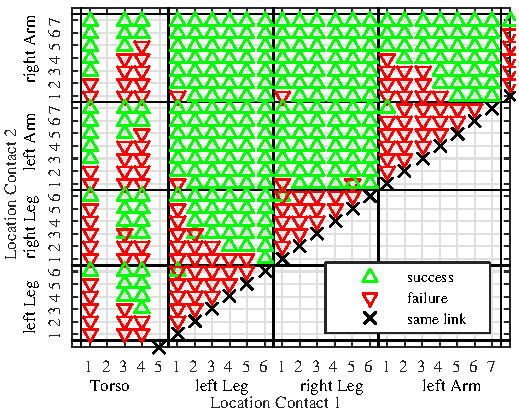
\includegraphics[width=\columnwidth]{figures/collest_multi_stat_2coll_rankmat/rankmat_fig_2coll_Modus2}
\end{center}\vspace*{-0.3cm}
\caption{Overview of success and failure for the isolation of two simultaneous contacts.
The $x$-axis gives the first contact link and the $y$-axis the second one.
The second and the last body of the torso chain have no collision body in the model, the according columns are therefore left empty.
A green upward triangle marks the successful isolation of both contact points for the given combination.
A red downward triangle marks a combination for which it was impossible to isolate the contacts correctly due to rank loss of the combined Jacobian in (\ref{eqn:multi_iso}).
In some fields, green and red triangles are plotted meaning that for this combination, the isolation was only partly correct.
For the combination of the fifth link in the right leg and the first link of the right arm, this is due to the fact, that for some contacts, the joint torque threshold for the last joint is not exceeded and the algorithm is therefore started with a loss of rank in the Jacobian.
However, when reducing the joint torque threshold or starting the algorithm with the correct contact links, this could not be observed anymore.
In the other cases, the contact point was estimated correctly by accident with a rank deficient Jacobian.
Overall 5000 combinations were tested.}\vspace*{-0.5cm}
\label{fig:coll_multicontact_rankJ}
\end{figure}

\begin{figure}
\vspace*{-0cm}
\begin{center}
% Um die Prozentangaben für Overpic zu generieren: Skript histogram_error_rank.m im Bildordner ausführen und aus Textausgaben entnehmen.
\begin{overpic}{figures/collest_multi_stat_2coll_error_rank/hist_rank_err_2coll}
\put(50,78){\line(2,0){10}}
\put(63,76){$100\%$}

\put(49,47){\line(2,3){8}}
\put(56,61){$34\%$}

\put(43,35){\line(1,1){15}}
\put(55,52){$21\%$}

\put(55,36){\line(2,1){7}}
\put(55,40){$11\%$}

\put(68,17){\line(1,1){15}}
\put(80,34){$2\%$}
\end{overpic}
\end{center}
\caption{Histogram of the maximum point estimation error for two contacts with different random contact configurations. Read: ``34\% of the results for $\mathrm{rank}(\bm{J})=11$ lie between 15 and 25~cm.''}
\label{fig:hist_rank_err_2coll}
\vspace*{-0.3cm}
\end{figure}

\subsubsection{Contacts at four end-effectors}

For the considered 30~DoF humanoid, it is possible to detect and isolate up to $N_\mathrm{C}=5$ contacts, if the rank deficit $RD$ is zero.
This is the case for four contacts at the end-effectors of every kinematic chain (feet, hands) and an additional contact located at the torso or first shoulder link, which is the typical manipulation scenario from Fig~\ref{fig:manip}.
The distribution of position errors for this case are depicted in Fig.~\ref{fig:error_rank_manipcoll} with markers for different rank deficits $RD$.

Without rank deficit, the isolation is successful in all but 5 of the 5000 examined points, where there was no rank deficit.
The errors occur in situations, where the joint torque threshold for the last joint in at least one chain is not exceeded.
This leads to a Jacobian with rank-deficit for the first iteration step of the algorithm, making it in a few cases impossible to find the correct contact link.
However, if the threshold is reduced to $10^{-5}$~N or Nm (for all  $\lVert\bm{f}_{\mathrm{ext},i}\rVert<1$), or the algorithm is started with perfect information about the contact links, no errors are observed.
The maximum and mean execution times for the isolation in this experiment were 0.92~ms and 0.52~ms using force/torque sensors as well as 43.2~ms and 11.0~ms using joint torque measurements only.

\begin{figure*}
\begin{center}
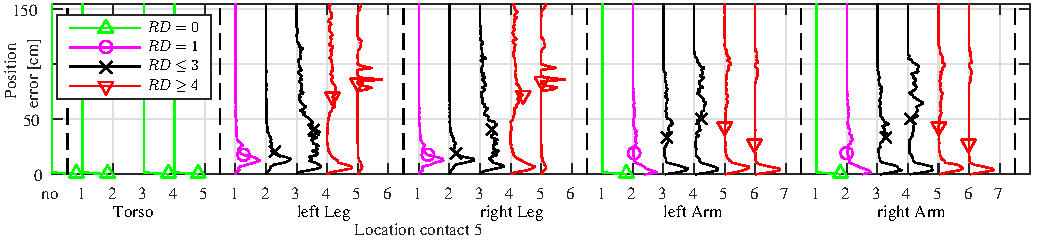
\includegraphics{figures/collest_multi_stat_manipcoll_error/error_rank_manipcoll_hist_breit}
\end{center}\vspace*{-0.4cm}
\caption{Distribution of the isolation position error based on joint torques only with contacts at all end-effectors for different rank deficits $RD$ of the Jacobian.
The position error distributions are drawn over the location for a fifth contact.
The fifth contact location can be none (only four contacts) or any of the links, which are not an end-effector link.
Therefore the four columns of the end-effectors are left empty.
The columns of the second and the last torso chain link are left empty, because their model does not have any contact bodies, making it impossible to place contacts at these links.
Markers in the lines denote the mean errors of all contact points including this link.
The distribution lines are normalized to the highest corresponding value of the distribution.}\vspace*{-0.7cm}
\label{fig:error_rank_manipcoll}
\end{figure*}

\subsubsection{Benefits of additional force/torque sensors}

The results show the benefits of supplementary force/torque sensors, see Table~\ref{tab:sensor_benefits}.
Without force/torque sensors, up to five contacts can be detected, isolated and identified correctly under certain conditions.
With force/torque sensors in the distal links, at least the generalized external manipulation and locomotion forces can be found and further contacts can be isolated by additional force/torque sensors (max. one per sensor) or the first method (up to 5 in theory).
%
\begin{table}
\caption{Possibilities of collision detection, isolation and identification with different numbers of force/torque sensors in the kinematic tree. The sensors are meant to be added up down the lines of the table.}\label{tab:sensor_benefits}
\begin{tabular}{|p{2.8cm}|p{5cm}|}
\hline
sensors & possibilities\\\hline
only joint torque and base movement sensors & identify ground contact and manipulation contacts, detect single collision, isolate and identify single collision under certain conditions (see Fig.~\ref{fig:error_rank_manipcoll})\\\hline
distal force/torque sensors & full elimination of ground contact and manipulation forces, detection isolation and identification of single collisions, multiple collisions can be detected, isolated and identified in many cases\\\hline
additional force/torque sensors in the kinematic chains & detect isolate and identify one additional contact wrench per additional sensor\\\hline
\end{tabular}\vspace*{-0.3cm}
\end{table}

\subsection{Time Series Analysis of a Single Contact}
The influence of the observer dynamics on the isolation and identification is investigated by using generalized external forces including observer dynamics.
The external force acts over a sinus half wave with an amplitude of one and a cycle time of 40~ms.
The observer is run at a sample frequency of 1000~Hz and $K_O=500$ as suggested in \cite{Haddadin2014}.
In this simulation, the observer error and the error in acceleration estimation for the force/torque sensor compensation are assumed to follow the dynamics presented in (\ref{eqn:obs_dynamic}) and (\ref{eqn:qDD_dyn}) respectively.
%
\begin{figure}
\begin{center}
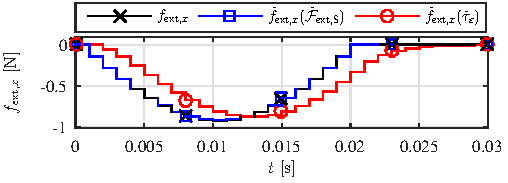
\includegraphics{figures/colltest_single_filter/colltest_single_filter_f}
\end{center}\vspace*{-0.4cm}
\caption{The $x$-component of the external force $\bm{f}_\mathrm{ext}$, the external force estimated with force/torque sensors  $\hat{\bm{f}}_{\mathrm{ext}}(\hat{\bm{\mathcal{F}}}_{\mathrm{ext,S}})$ according to (\ref{eqn:cmp}) and (\ref{eqn:cmp_ext_vorher}) as well as the external force estimated with the observed generalized forces $\hat{\bm{f}}_{\mathrm{ext}}(\hat{\tau}_\epsilon)$ according to (\ref{eqn:force_identification}) is depicted over time for a collision of  20~ms.
When using the generalized forces for identification, the estimated external force is a first order filtered version of the real force with time constant $K_O^{-1}$.
Using compensated force/torque sensors, the estimated force follows the real force without any delay.}\vspace*{-0.6cm}
\label{fig:coll_singlecontact_filter}
\end{figure}
%
With both methods described before, the contact point is isolated correctly up to numerical errors.
If the observed generalized joint forces are used for isolation, there is a delay of one time step, as the filtered generalized forces are still zero for the first time step of the collision.

Fig.~\ref{fig:coll_singlecontact_filter} shows the external forces over the collision time and the forces identified with and without the use of force/torque sensors.
It can be seen that if no force/torque sensors are used, the contact force is estimated with a delay of approximately 3~ms.
It has to be noted, that the collision will be seen about 10~ms longer with the observer dynamics taken into account.
This timespan depends on the thresholds for the generalized external forces, which was here chosen to be 0.001~N or 0.001~Nm, respectively and the filter frequency $1/K_O$.
Furthermore, when using force/torque sensors, smaller delay but larger error in the estimated external force can be observed.
As the error of $\hat{\ddot{\bm{q}}}$ is driven by $\bm{\tau}_\mathrm{ext}$ and $\bm{M}(\bm{q})$ is nearly constant for the robot at standstill, the contact point can still be estimated correctly with the compensated force/torque sensor.



% \addtolength{\textheight}{-12cm}   % This command serves to balance the column lengths
                                  % on the last page of the document manually. It shortens
                                  % the textheight of the last page by a suitable amount.
                                  % This command does not take effect until the next page
                                  % so it should come on the page before the last. Make
                                  % sure that you do not shorten the textheight too much.

% !TEX root = collhdl_ICRA_17.tex

\section{Conclusion}
\label{sec:conclusion}
In this paper, we propose a unified framework for collision detection, isolation and identification of generalized external forces acting along a humanoid robot.
Apart from standard proprioceptive sensing, the proposed scheme makes use of joint torque measurements and acceleration estimates.
Noticeably, it is shown how a generalized momentum observer may be used to calculate these quantities.
As the consequential next step, information from load-compensated force/torque sensors, which can be located arbitrarily along the robot structure, is integrated.
Considering ideal measurements it is shown that estimating the position of a single contact for humanoid robots is possible without any additional sensors.
The positions of multiple concurrent contacts may be estimated with additional force/torque sensors, or, under certain conditions, even without additional sensors.

Future work will cover analyzing the robustness of our scheme in more realistic simulations, in particular with respect to model uncertainties and sensor noise, as well as real world setups.
Also, the complexity and execution time of the algorithm on a real-time enabled system has to be examined closely.
Furthermore, we will investigate the further systematic fusion of joint torque and force/torque sensing in the collision handling context.
Other open questions relate to the thorough yet practical handling of contacts with external moments such as surface contacts and dealing with singularities.

%%%%%%%%%%%%%%%%%%%%%%%%%%%%%%%%%%%%%%%%%%%%%%%%%%%%%%%%%%%%%%%%%%%%%%%%%%%%%%%%%
%\section*{APPENDIX}
%
%% Appendixes should appear before the acknowledgment.


%\section*{ACKNOWLEDGMENT}

\renewcommand{\baselinestretch}{0.86}
% % BIBLIOGRAPHY
\bibliographystyle{abbrv}
% \bibliographystyle{plain}
\bibliography{references}

\end{document}
	